\documentclass[cyan]{YuNote}

\begin{document}
\tableofcontents
\chapter{Introduction}
The field of of pattern recognition is concerned with the automatic discovery of regularities in data through the use of computer algorithms and with the use of the regularities to take actions such as classifying the data into different categories.

\section{Handwritten digits recognition} 

\begin{figure}[!hbtp]
\center
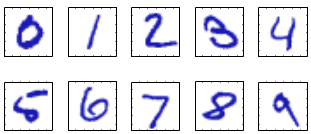
\includegraphics[width=0.6\textwidth]{figure1_1.png}
\caption{美国邮件上的手写数字样本}
\end{figure}

\subsection{empirical approach}
\begin{newpara}
hand-crafted rules or \stressB{heuristics} for distinguishing the digits based on the shapes of the strokes.\\
使用手工编写的规则或者是\stressB{启发} 来通过笔画的形状鉴别阿拉伯数字。
\end{newpara}

\stressA{Proliferation of rules and poor results.}
\subsection{machine learning approach}
\begin{itemize}
\item$N$位的\trans{训练集}{tanning set} $\lbrace x_1,\ldots,x_N\rbrace$
\item \trans{目标向量}{target vector}来表示每训练集元素对应的类别(0-9)
\item \trans{训练过程}{tanning phase}确定了函数$\textbf{y}(x)$
\end{itemize}


\section{Example:Polynomial Curve Fitting}
\begin{equation}
y(x,\textbf{w})=w_0+w_1+w_2x^2+\ldots+w_Mx^M=\sum_{j=0}^M w_jx^j
\end{equation}


\begin{equation}
E(\textbf{w}) =\dfrac{1}{2} \sum_{n=1}^N y \lbrace (x_n,\textbf{w})-t_n\rbrace^2
\end{equation}

\begin{equation}[Definition:$RMS$]
E_{RMS}=\sqrt{2E(\textbf{w}^*)/N}
\end{equation}

\begin{equation}
\tilde{E}(\textbf{w})=\dfrac{1}{2}\lbrace y(x_n,\textbf{w})-t_n\rbrace^2+\dfrac{\lambda}{2}\Vert\textbf{w}\Vert^2
\end{equation}
\section{Probablility Theory}
The rules of Probability
\begin{equation}[sum rule]
p(X)=\sum_Y p(X,Y)
\end{equation}

\begin{equation}[product rule]
p(X,Y)=p(Y|X)p(X)
\end{equation}
\begin{equation}[Bayes'theorem]
p(Y|X)=\dfrac{p(X|Y)p(Y)}{p(X)}
\end{equation}
\begin{equation}[贝叶斯推论]
P(X)=\sum _Y p(X|Y)p(Y)
\end{equation}
\begin{note}
可以看成原始两边对$Y$累加,然后左边$P(Y|X)$项累加和等于1约去
\end{note}
\subsection{Probability densities}
\begin{equation}[$x$上$(a,b)$区间内的概率密度]
p(x\in(a,b))=\int _a^b p(x)dx
\end{equation}
\trans{概率密度}{probability density}$p(x)$必须满足的两个条件\\

\begin{equation}[1.]
p(x) \geqslant 0
\end{equation}
\begin{equation}[2.]
\int_{-\infty}^{\infty}p(x)dx=1
\end{equation}
\begin{equation}
\begin{split}
p_y(y)&=p_x(x)\vert\dfrac{dx}{dy}\vert\\&=p_x(g(y))\vert g'(y)\vert
\end{split}
\end{equation}
\begin{note}
额。。。。暂时没看懂
\end{note}
在$(-\infty,z)$区间内的\trans{概率分布函数}{cumulative distribution function}定义如下:\\
\begin{equation}
P(z)=\int_{-\infty}^zp(x)dx
\end{equation}
\begin{note}
满足了$P'(x)=p(x)$
\end{note}
当有多个连续的自变量$x_1,\ldots,x_D$时,将其整体表示为$\mathbf{x}$,于是可以定义一个联合的概率密度函数$p(\mathbf{x})=p(x_1,\ldots,x_D)$于是有了以下两个条件:\\
\begin{equation}[1.]
p(\mathbf{x}) \geqslant 0
\end{equation}
\begin{equation}[2.]
\int_{-\infty}^{\infty}p(\mathbf{x})d\mathbf{x}=1
\end{equation}
如果$x$是一个离散的变量,$p(x)$就被叫做\trans{概率质量函数}{probability mass function}\\
\begin{equation}
p(x)=\int p(x,y)dy
\end{equation}
\begin{equation}
p(x,y)=p(y|x)p(x)
\end{equation}

\subsection{Expectations and covariances}
在概率分布$p(x)$下的某些函数$f(x)$的平均值叫做$f(x)$的\trans{期望}{expectation},标记为$\mathbb{E }[f]$\\
离散分布下期望定义为:
\begin{equation}[离散分布期望定义]
\mathbb{E}[f]=\sum_xp(x)f(x)
\end{equation}
连续分布下期望定义为:
\begin{equation}[连续分布期望定义]
\mathbb{E}[f]=\int p(x)f(x)dx
\end{equation}
\end{document}

